\section{Experiments}\label{sec:expts}

\begin{table}
\begin{tabularx}{\textwidth}{| p{1.9cm} | X | X | X | X | X | X | X | X |}
\hline
Dataset & Folds /subs-amples & Users & Items & Pairs, train & Pairs, test & Pref vals, test & Item features & User features \\
\hline\hline
Simulation (a) & 25 & 25 & 100 & 900 & 0  & 100 & 2 & 2\\
Simulation (b) & 25 & 25 & 100 & 900 & 0 & 100 & 2 & 2 \\
Simulation (c) & 25 & 25 & 100 & 900 & 0 & 100 & 2 & 2\\
Simulation (d) & 25 & 25 & 100 & 36 - 2304 & 0 & 100 & 2 & 2\\
\hline
Sushi A & 25 & 1000 & 10 & 15000 & 5000 & 10000 & 18 & 123 \\
Sushi B & 25 & 5000 & 100 & 50000 & 5000 & 500000 &  18 & 123 \\
\hline
UKPConvArg-CrowdSample & 32 & 1442 & 1052 & 16398 & 529 & 33 & 32310 & 0
\\ \hline
\end{tabularx}
\caption{Summary of datasets showing mean counts per subsample or per fold. For the simulation datasets, generate the subsamples of data independently, for the Sushi dataset we select subsamples independently from the complete dataset, while  
UKPConvArgCrowdSample is divided into folds, where the test data in each fold corresponds to a single topic and stance. The numbers of features are given after categorical labels have been converted to one-hot encoding, counting
each category as a separate feature.
}
\label{tab:datasets}
\end{table}
% NOTE: possible problem with convincingness data is that some users have very few observations in training data.
We use the datasets summarized in Table \ref{tab:datasets} to test the key aspects of our proposed methods: recovering an underlying consensus from noisy pairwise labels; modeling personal preferences from pairwise labels; and the scalability of our proposed Bayesian preference learning methods, GPPL and crowd-GPPL using SVI.
In Section \ref{sec:exp_synth}, we use simulated data to test the ability of our method to recover preference functions from noisy data when the correct number of latent factors is unknown. 
Then, in Section \ref{sec:sushi}, we compare our method against previous approaches for predicting the preferences
of thousands of users on the \emph{Sushi} datasets~\citep{kamishima2003nantonac}.
Section \ref{sec:exp_nlp} evaluates our approach on an NLP task with high-dimensional feature vectors and
a larger number of items, which involves using pairwise judgments of arguments from online debate forums 
to learn a function of argument \emph{convincingness}. We use the \emph{UKPConvArgSample} dataset, which is 
sampled from data provided by ~\citet{habernal2016argument}. 
Finally, we analyze the scalability of our SVI approach in Section \ref{sec:exp_scale}, again using the \emph{UKPConvArgSample} dataset.

\subsection{Methods Compared}

We refer to the multi-user variant of our model as \emph{crowd-GPPL}.
As baselines, we use GPPL to learn a single preference function from all users' preference labels, (\emph{GPPL-pooled}), and a Gaussian process over the joint feature space of users and items 
(\emph{GPPL-joint}), as proposed by \citet{guo2010gaussian}.
For datasets up to 100 users (simulated data, subsamples of the real datasets), 
we also test separate GPPL instances per user with no collaborative
learning (\emph{GPPL-per-user}), but this could not be applied to the real datasets as the 
computation costs were too high.
To test the benefit of using GPs to model item and user features,
we also test two further baselines: 
\emph{crowd-GPPL$\mathbf{\setminus \bs u}$}, which ignores the user features,
and \emph{crowd-BMF}, which ignores both user and item features and so does not use GPs at all. 
For both of these methods, the user covariance matrix, $\bs K_w$, in the crowd-GPPL model is replaced by the identity matrix, and for \emph{crowd-BMF}, the item covariance matrices, $\bs K_v$ and $\bs K_t$ are also replaced by the identity matrix.

% Ranking-SVM baseline -- only easy to compare in the single user case. My GPPL paper perhaps needs
% this adding in any follow up works.

% Houlsby tests: with/without user features (without is better with few users). + a hierarchical 
% model, BI (multi task preference learning, Birlitiu et al), and the GPPL-joint model. None of 
% these are done at scale, which we can do with our inference method --> *this is a new claim i.e. 
% new empirical results*. They also test a per-user model.

\subsection{Simulated Noisy Data}\label{sec:exp_synth}

First, we test how well GPPL is able to recover an underlying consensus function
in the presence of varying amounts of noise.

We generate data by first selecting $100$ points at random
from a $10x10$ 2-dimensional grid and choosing $500$ pairs of these points at random. 
We generate pairwise labels by drawing from the single user GPPL model:
first, draw latent preference function values for the selected points; 
then, compute the pairwise likelihoods for the selected pairs using Equation \ref{eq:plphi};
draw pairwise labels from the Bernoulli likelihoods. 
We split the chosen points into 50\% training and test sets, and
train GPPL on all pairs involving only points in the training set.
We then use GPPL to latent predict preference function for the points in the test set.
We repeat this process, varying the value of $s$ in the generation step, 
which controls the precision of a latent preference function: as $s$ is increased, the latent
function values have a smaller amplitude and the pairwise labels become noisier.
The hyper-parameters of the GPPL model for prediction remain the same throughout, 
with $\alpha_0 = 2$, $\beta_0 = 2$.
We repeat the complete experiment $25$ times, including generating new data for each value of $s$.

The results of the first test in Figure \ref{fig:simA} show that increasing
the noise rate in the pairwise labels causes a near-linear decrease in the
rank correlation between the predicted and true preference function values. 
Nonetheless, GPPL is able to recover the ranking of points with $\tau > 0.5$ when
more than $1/3$ pairwise labels are incorrect.

In the second simulation, we recover a consensus function
from preference labels produced by multiple simulated users with varying differences
in their individual preferences. We use the same process as the first simulation, except
we now draw the pairwise labels from a crowd-GPPL model with $25$ users and $3$ latent factors,
instead of a single-user model. We fix the inverse scale of the latent item factors, $s=0.001$,
but vary the precision of the consensus function, $\sigma$. 
We use three methods to recover the consensus function: \emph{GPPL-per-user},
in which an independent model is trained for each user, and the mean of their
predictions is used to estimate the consensus; 
\emph{pooled-GPPL}, a single instance of GPPL trained on pairwise labels from all users; 
and crowd-GPPL, with $C=25$ so that there is one factor per user. 

Figure \ref{fig:simB} shows that the crowd-GPPL model is better able recover the latent consensus
function than the other methods, even when noise levels are high. 
The pooled model's predictions may be worsened by biased users whose preferences deviate
 consistently from the consensus. GPPL-per-user relies on separate instances of GPPL, so 
 does not benefit from sharing information between users when training the model.

The third test repeats a similar setup to the second, but here we evaluate the methods'
ability to to recover the personal preferences of individual simulated users.
We fix $\sigma = 10$ and vary the precision of the item latent factors, $s$.

Results for predicting personal preferences in the presence of noise are shown in 
Figure \ref{fig:simC}. Crowd-GPPL is able to make better predictions when noise is below
$0.3$ but its benefit disappears when the noise level increases further. 

In the final simulation, we evaluate the effect of the quantity of training data 
in scenarios with different numbers of latent factors.
We hypothesized that a larger number of latent factors would indicate a more complex
scenario that would require more training data. 
We generate data again from the crowd-GPPL model with $s=0.2$ and $\sigma=1$
and vary the number of true latent factors using values $C_{true} \in \{ 1, 3, 10, 20\}$.
For each value of $C_{true}$, we run crowd-GPPL with increasing numbers of pairwise labels,
and evaluate the correlation between inferred and true latent user factors. 
To match inferred factors to true factors, we compute Pearson correlations between each
true factor and each inferred factor, then repeatedly select the pair of unmatched 
factors with the highest correlation as a new match until all true factors are matched. 

The results in Figure \ref{fig:simD} show that...

\begin{figure}
\subfloat[Inferring preferences for a single user]{
\label{fig:simA}
\includegraphics[width=.5\columnwidth]{../../results/synth_3/single_user/tau_test}
}
\subfloat[Inferring consensus function from crowdsourced labels]{
\label{fig:simB}
\includegraphics[width=.5\columnwidth]{../../results/synth_3/multi_user_consensus/tau_test}
} \\
\subfloat[Inferring personal preferences for members of a crowd]{
\label{fig:simC}
\includegraphics[width=.57\columnwidth]{../../results/synth_3/multi_user_personal/tau_test}
}
\subfloat[Inferring the latent factors]{
\label{fig:simD}
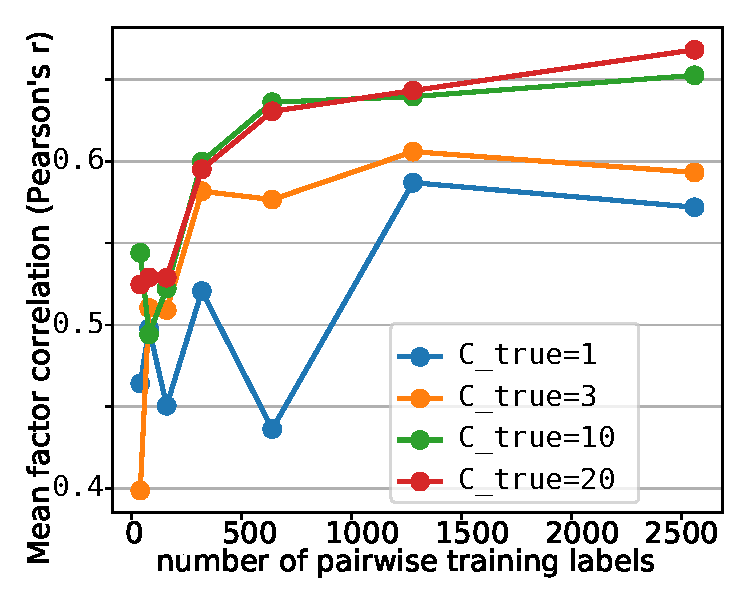
\includegraphics[width=.43\columnwidth]{../../results/synth_3/multi_factor_correlations_P/num_pairs_r}
}
\caption{Rank correlation between true and inferred preference values for different inference tasks.  (a)--(c) varying level of noise in pairwise training labels, (d) varying number of pairwise training labels. 
}
\end{figure}


\subsection{Sushi Preferences}\label{sec:sushi}

Dataset: Sushi
% Houlsby results: for comparison against a different inference technique on small data, include
% the test error results from their paper.
% Guo results: not directly comparable. We will rerun a similar approach but with our inference method.
% Khan results: for a different model that separates the latent features from the item/user features.
% Abbasnejad results (community-based preference learning): sushi data with 10 items; 60/40 train/test split of each user's preference pairs. This means the result is based on 27 pairs training.
% don't worry about this though, it doesn't seem to work very well in their results.

Hypothesis: 
% Number of users affects value of including user features.
% Plot results on increasing dataset size.

% [10] T. Kamishima. Nantonac collaborative filtering:
% Recommendation based on order responses. In
% ACM SIGKDD 9th Int. Conf. Knowledge Discov-
% ery and Data Mining, 2003.

Setup:

Run 25 repeats of random train/test splits with:
% Exclude these two as we focus on bigger datasets in this paper. Cutting these creates the space 
% for including three metrics.
% Downside: cannot test whether increasing no. users imroves performance through better collaborative learning. 
% 
% 100 (a la Houlsby 20 pairs per user), 
% 200 (a la Khan, 3 training, 1 test, P=600, P_test=200), 
% For small datasets, we may want to test on the argumentation data so we can assess the crowd
% consensus results with small data. That dataset is more interesting here because lots of items,
% small data is a new scenario.
[a] 1000 (a la Houlsby 15 training, 5 test pairs per user, $P=15000,P_{test}=5000$), Sushi-A (10 items), 
and [b] 5000 users (a la Khan, 10 training, 1 test pairs per user, $P=50000, P_{test}=5000$), Sushi-B (100 items).
Evaluate on parwise labelling error, pairwise label logloss, spearman rank correlation,
and runtime.
% could use normalized mean loss from guo, but not sure where the utilities come from -- ranking?

% 25 random train/test splits on all 5000 users with varying no. (1, 5, 10, 20, 40) pairs per user.

% Can put in the Houlsby (100/1000 users, 20 pairs each, labelling error) and Khan (200 users, 3 pairs each, logloss) results.
% Khan also provide code, so could be rerun to get classification error.

% Also consider whether we can show more results in a table format?

In all cases, we use the no. pairs per user and no. users to select the subset of data used for training, then test on the remainder.

\begin{table}
\begin{tabularx}{\textwidth}{| l | c | c | c | c |}
\\ \hline
%\input{../../results/sushi_10_4/results.tex}\\
%\input{../../results/sushi_10_opt_4/results.tex}\\
\\ \hline
\end{tabularx}
\caption{Performance on Sushi-A dataset with 10 items, 1000 users, 15 pairwise labels per user for training.}
\end{table}

\begin{table}
\begin{tabularx}{\textwidth}{| l | c | c | c | c |}
\\ \hline
%\input{../../results/sushi_100_4/results.tex} \\ 
%\input{../../results/sushi_100_opt_4/results.tex} \\
\\ \hline
\end{tabularx}
\caption{Performance on Sushi-B dataset with 100 items, 5000 users, 10 pairwise labels per user for training.}
\end{table}

\begin{figure}
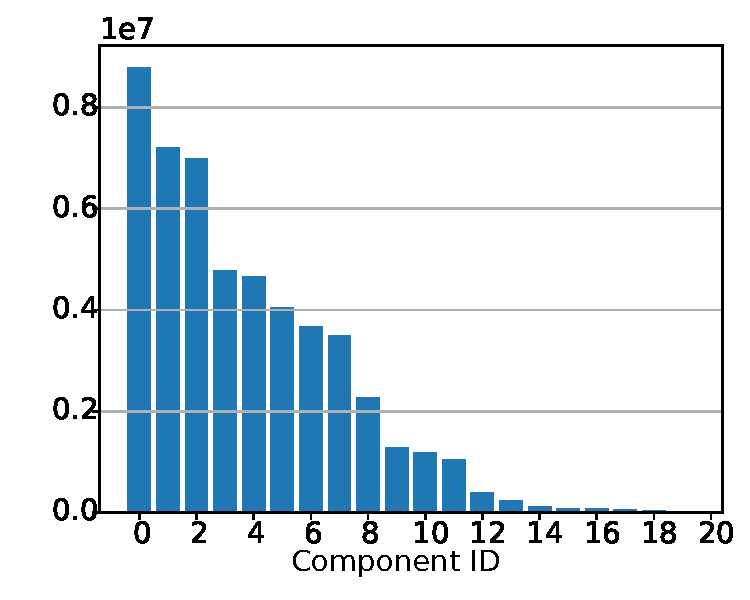
\includegraphics[scale=1]{../../results/sushi_factor_scales}
\caption{
Distribution of latent factor variances, $s_c$, for crowd-GPPL on the Sushi-A and Sushi-B datasets, averaged over all $25$ runs.
}
\end{figure}

\subsection{Argument Convincingness}\label{sec:exp_nlp}

We compare performance of several methods on the Dataset used in Section \ref{sec:exp_scale}.

The judgments were obtained by asking crowdsourcing workers to decide which of a pair of arguments is 
more convincing. The dataset contains 16 debate topics, each of which has two stances and
contains consensus judgements as well as 
The data comes from ...
We use this dataset to evaluate performance in a high-dimensional problem with $32,310$ feature dimensions.
These features include ...
Single-user GPPL was tested on this dataset in . Here we test the benefits of
the crowd-GPPL model for predicting the consensus and test both single-user and crowd-GPPL for predicting
the individual preferences of workers in the crowd.
The datasets are 

Methods: 

Hypothesis: 


\begin{table}
\begin{tabularx}{\columnwidth}{ | l | X | X | X | X | X | X |}
\hline
 & \multicolumn{3}{|X|}{Consensus}&\multicolumn{3}{| X |}{Personal} \\ \hline
 Method & Acc & CEE & Kend. & Acc & CEE & Kend. \\ \hline
 SVM & .70 & .58 & .31 & .63 & .66 & .31 \\
 Bi-LSTM & .73 &  .55 & .21 & .64 & .64 & .21 \\
 GPPL medi. & \textbf{.77} & \textbf{.50} &  \textbf{.40} & .69 & .59 & .40 \\
 GPPL opt. & & & & & &  \\
 Crowd-GPPL medi. & & & & & & \\
 Crowd-GPPL opt. & & & & & & \\
 PL+ SVR & .75 & .55 & \textbf{.40} & .75 & & .40 \\
 GPC & .73 & .53 & - & .68 & .59 & - \\
 \\\hline
\end{tabularx}
\caption{Performance comparison on UKPConvArgCrowdSample using ling+GloVe features. \emph{Acc} and \emph{CEE} show classification accuracy and cross entropy error (or log-loss) for pairwise predictions, 
while \emph{Kend.} shows Kendall's tau for the predicted preference function.}
\label{tab:convarg}
\end{table}

\begin{figure}
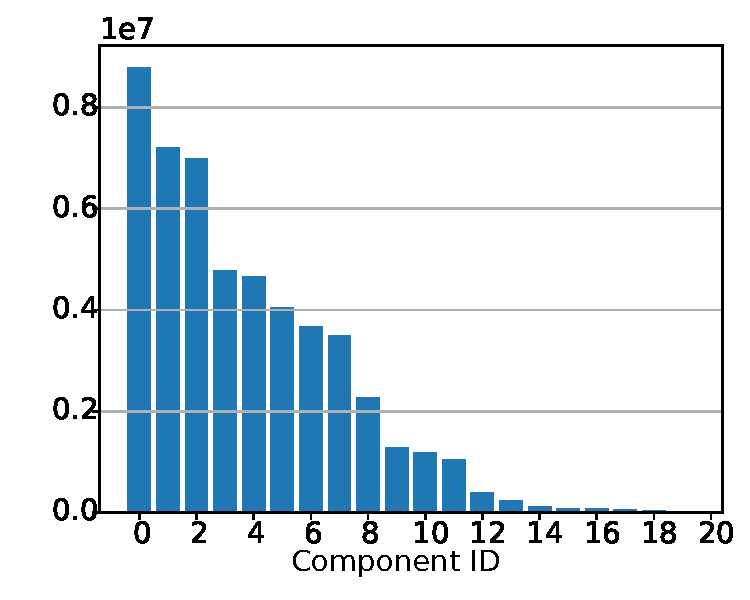
\includegraphics[scale=1]{../../results/sushi_factor_scales}
\caption{
Distribution of latent factor variances, $s_c$, for crowd-GPPL on UKPConvArgCrowdSample, averaged over all $32$ runs.
}
\end{figure}

\subsection{Scalability Experiments}\label{sec:exp_scale}

Dataset:

Hypothesis: 

List of experiments to include -- need new plots for the crowd model:
\begin{enumerate}
\item Performance, computation time vs. no. inducing points
\item Computation time vs. dataset size, no. features
%\item not done: memory vs no. inducing points, update size
%\item not done: Performance, computation time, vs update size
%%\item not done: performance, computation time vs different initialisation methods for the inducing points; include different initialisations of K-means
\end{enumerate}

\begin{figure}
\subfloat[Varying number of items in training set. GloVe features.]{
    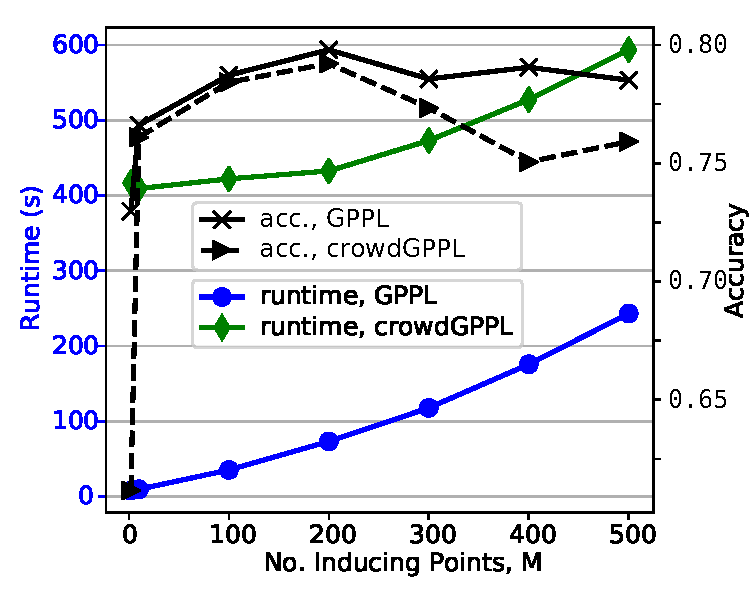
\includegraphics[scale=1]{../../results/scalability/num_inducing_32310_features}
}
\subfloat[Varying no. ling+GloVe features. $M=500$]{
    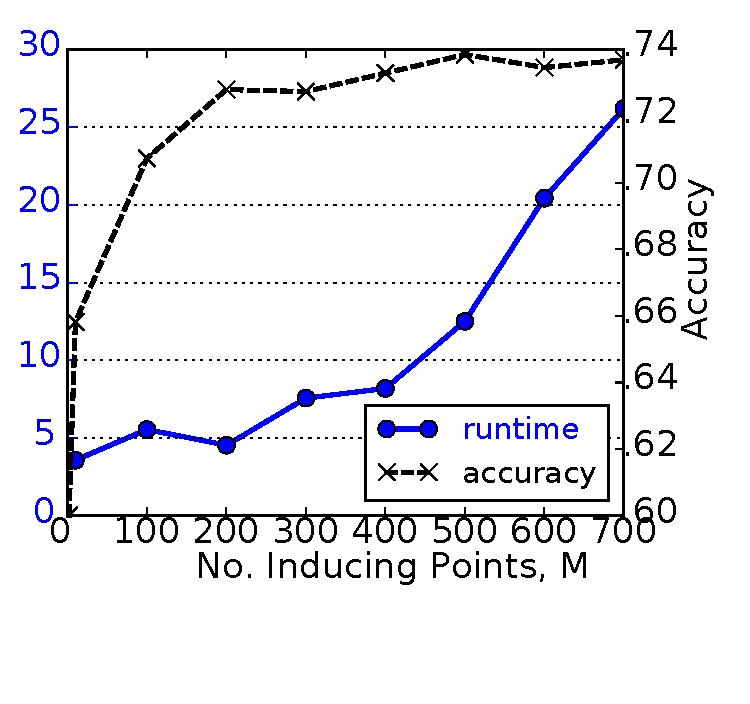
\includegraphics[scale=1]{../../results/scalability/num_inducing_300_features}
}
\caption{
    Runtimes for training+prediction on UKPConvArgCrowdSample with varying subsample size. Means over 32 runs. 
    Note the logarithmic x-axis for (b).
}
\end{figure}
\begin{figure}
\subfloat[33210 ling+GloVe features]{
    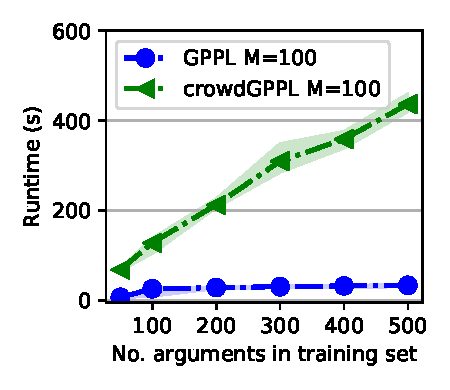
\includegraphics[scale=1]{../../results/scalability/num_arguments}
}
\subfloat[300 GloVe features]{
    \includegraphics[scale=1]{../../results/scalability/num_features}
}
\caption{
Effect of varying $M$ on accuracy and runtime (training+prediction) for GPPL and crowd-GPPL on UKPConvArgCrowdSample. Means over 32 runs.
}
\end{figure}
